\chapter{Architecture Study}\label{Study1}

This study's main purpose is to figure out how suited each architecture is for \acrfull{ADT}, more specifically \acrfull{DTM} tasks. This could help us figure out which architecture is superior for \gls{ADT}, if there are any similarities between architectures who perform similarly well, or if there are any architectures who perform poorly.

\section{Methodology}

We perform hyperparameter tuning and model selection to train a separate model for each architecture over each dataset. At last we test the model on each dataset's respective test split. As a result, we are left with performance measures on unseen data from the same distribution as those each model was train on. This will give us a good intuition into each architecture's ability to learn the task of \gls{ADT} and could help us estimate their generalization ability.

\section{Results}	

\begin{table}[H]
    \centering
    \hspace*{-0.6cm}
    \begin{tabular}{l|cccc}
        Architecture & ENST+MDB & E-GMD & Slakh & ADTOF-YT       \\
        \hline
        Recurrent Neural Network	& 0.67 &	 &	0.86 &	\textbf{0.96} \\
        Convolutional Neural Network	& 0.78 &	 &	0.83 &	0.84 \\
        Convolutional Recurrent Neural Network	& \textbf{0.81} &	 &	\textbf{0.90} &	0.93 \\
        Convolutional Transformer	& 0.77 &	 &	0.88 &	0.95 \\
        Vision Transformer	& 0.54 &	 &	0.88 &	\textbf{0.96} \\
        
    \end{tabular}
    \caption{The Micro F1-score for each architecture, trained and tested on each dataset. The performances which are \textbf{bolded} represent the highest F1-score, and thus best performance, for that respective dataset.}
    \label{ArchitectureResultsTable}
\end{table}


\begin{figure}[H]
    \centering
    \hspace*{-0.8cm}
    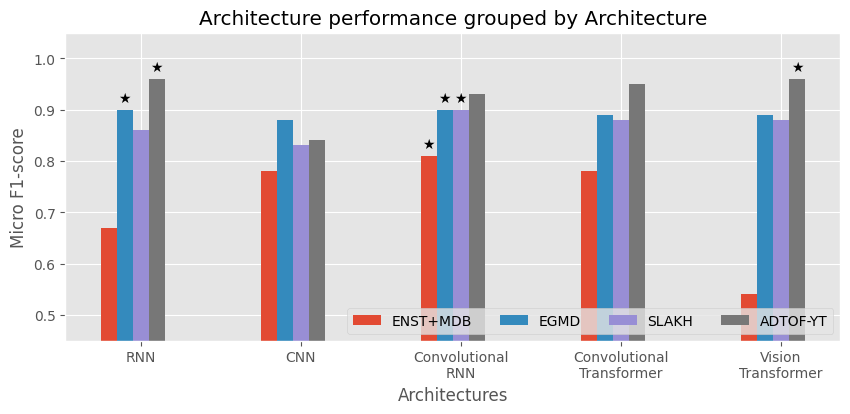
\includegraphics[scale=0.8]{figures/architectureperformancearchitecture.png}
    \caption{Comparison of Micro F1-scores for each dataset across the different architectures. Bars marked with a ($\star$) indicate the best performing architecture for each respective dataset.}
    \label{ArchitectureResultsArchitectureFigure}
\end{figure}

\begin{figure}[H]
    \centering
    \hspace*{-0.8cm}
    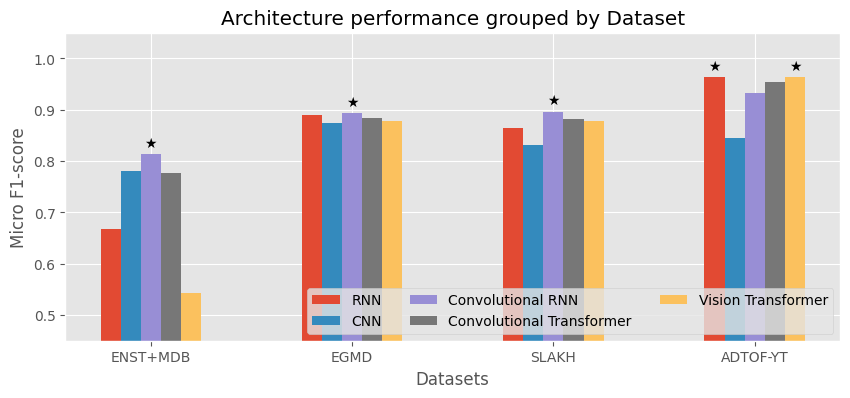
\includegraphics[scale=0.8]{figures/architectureperformancedataset.png}
    \caption{Comparison of Micro F1-scores for each architectures across the different dataset. Bars marked with a ($\star$) indicate the best performing architecture for each respective dataset.}
    \label{ArchitectureResultsDatasetFigure}
\end{figure}

\section{Discussion}

The results from the architecture study, summarized in Table \ref{ArchitectureResultsTable} and Figures \ref{ArchitectureResultsArchitectureFigure} and \ref{ArchitectureResultsDatasetFigure}, indicate that there is no single superior architecture for \gls{ADT}. Instead, performance is variant on the properties of each dataset, as well as the inherent inductive biases of each architecture.

Firstly, it is evident that there does not seem to be one superior architecture when it comes to \gls{ADT}. There does not exist a single architecture outperforming the others across all the datasets, and the different architectures often share similarly high performances on most of the datasets. 

However, the convolutional recurrent neural network demonstrates the highest Micro F1-score on three of the four datasets (namely ENST+MDB, E-GMD and Slakh). It also provides a high, but not exceptional F1-score on the fourth (ADTOF-YT). The consistency of its high performance across the different characteristics of each dataset suggests that it is able to handle a wide variety of \gls{ADT} tasks, and that its performance may be high independent on the training dataset's size and complexity. In other words, it displays properties of being a architecture highly suitable for \gls{ADT} tasks. One could speculate that this suitability is provided by the strong inductive bias from the combination of convolutions and recurrent units, allowing for both initial spatial feature extraction as well as short-range temporal modelling.

The convolutional neural network displays a moderate performance across all datasets. It shows adequate performance on the smallest dataset (ENST+MDB), having the second highest F1-score. However, across all others (E-GMD, Slakh and ADTOF-YT) it displays the lowest. This relatively poor overall performance seems to indicate that the convolutional neural network currently is an inferior architecture for \gls{ADT} tasks, unless dataset size is limited, in which it could provide a viable architecture. It also shows the importance of explicitly leveraging the temporal dependencies within \gls{ADT}, as solely relying on the inductive bias of the convolutions didn't prove sufficient here.

This importance seems to be strengthened by the performance of the purely recurrent neural network, which has a surprisingly high performance across the datasets. In a way, it displays the opposite behaviour compared to the \gls{CNN}, displaying inadequate performance for the smallest dataset (ENST+MDB), but a relatively high performance for two of the others (E-GMD and Slakh), sharing the crown for the highest F1-score on the last (ADTOF-YT). The first dataset's low performance suggests that the inductive bias of the recurrent layers are "weaker" than the ones from convolutions, relying on a larger amount of data to accurately learn the task. Notably, it significantly outperforms the \gls{CRNN} on the last dataset, hinting that the inductive bias of the convolutions might "overpower" the model, proving so strong that it ends up hindering its performance.

The convolutional transformers exhibits performance comparable to something in between the \gls{RNN} and \gls{CRNN}, and shows what can be described as the most consistent relatively high performance across all the four datasets. It puts itself just under the \gls{CRNN} for the first three datasets (ENST+MDB, E-GMD and Slakh), and a good step over for the last (ADTOF-YT). This does seem to indicate that the transformer models provide enough of a temporal inductive bias to accurately perform well on \gls{ADT} tasks, however it might also hint that the long range dependencies are more easily modelled with attention layers are not as important as the accurate short range aggregation from the recurrent layers on most \gls{ADT} datasets. Although by the performance displayed, the convolutional transformer could be chosen as a viable architecture for \gls{ADT}.

At last we have the vision transformer, which performs similar to the \gls{RNN}. For the smallest dataset (ENST+MDB) it displays a subpar performance with by far the lowest F1-score. For the two middle ones (E-GMD and Slakh) it exhibits a relatively average performance. For the last dataset (ADTOF-YT) it shows excellent performance, having an identical F1-score to the \gls{RNN}. This seems to agree with the previous conclusion that the inductive bias of the convolutional layers are "strong", putting a higher responsibility on a large amount of quality data when omitting it. The significantly poor performance on the small dataset might also indicate that the attention layers and transformer blocks come with an even "weaker" inductive bias than the recurrent layers, hightening the reliance on data amount. This aligns well with existing literature, where vision transformers generally require extensive training data or pre-training on larger datasets to obtain optimal performance~\cite{dosovitskiy2021imageworth16x16words}.

In summary, our results strongly indicate that the Convolutional Recurrent Neural Network is the current most suited architecture for \gls{ADT} tasks across different datasets. However, further research should be done into both the Vision Transformer and Recurrent Neural Network, gauging how these models scale with larger datasets.

\textcolor{red}{Is it relevant to talk about future research here or should it be in the final conclusion?}